% Размер страницы и шрифта
\documentclass[12pt,a4paper]{article}

%% Работа с русским языком
\usepackage{cmap}                   % поиск в PDF
\usepackage{mathtext}               % русские буквы в формулах
\usepackage[T2A]{fontenc}           % кодировка
\usepackage[utf8]{inputenc}         % кодировка исходного текста
\usepackage[english,russian]{babel} % локализация и переносы

%% Изменяем размер полей
\usepackage[top=0.5in, bottom=0.75in, left=0.625in, right=0.625in]{geometry}

%% Различные пакеты для работы с математикой
\usepackage{mathtools}  % Тот же amsmath, только с некоторыми поправками
\usepackage{amssymb}    % Математические символы
\usepackage{amsthm}     % Пакет для написания теорем
\usepackage{amstext}
\usepackage{array}
\usepackage{amsfonts}
\usepackage{icomma}     % "Умная" запятая: $0,2$ --- число, $0, 2$ --- перечисление

%% Графика
\usepackage[pdftex]{graphicx}
\graphicspath{{images/}}

%% Прочие пакеты
\usepackage{listings}               % Пакет для написания кода на каком-то языке программирования
\usepackage{algorithm}              % Пакет для написания алгоритмов
\usepackage[noend]{algpseudocode}   % Подключает псевдокод, отключает end if и иже с ними
\usepackage{indentfirst}            % Начало текста с красной строки
\usepackage[colorlinks=true, urlcolor=blue]{hyperref}   % Ссылки
\usepackage{pgfplots}               % Графики
\pgfplotsset{compat=1.12}
\usepackage{forest}                 % Деревья
\usepackage{titlesec}               % Изменение формата заголовков
\usepackage[normalem]{ulem}         % Для зачёркиваний
\usepackage[autocite=footnote]{biblatex}    % Кавычки для цитат и прочее
\usepackage[makeroom]{cancel}       % И снова зачёркивание (на этот раз косое)

% Изменим формат \section и \subsection:
\titleformat{\section}
	{\vspace{1cm}\centering\LARGE\bfseries} % Стиль заголовка
	{}                                      % префикс
	{0pt}                                   % Расстояние между префиксом и заголовком
	{}                                      % Как отображается префикс
\titleformat{\subsection}                   	% Аналогично для \subsection
	{\Large\bfseries}
	{}
	{0pt}
	{}

% Поправленный вид lstlisting
\lstset { %
    backgroundcolor=\color{black!5}, % set backgroundcolor
    basicstyle=\footnotesize,% basic font setting
}

% Теоремы и утверждения. В комменте указываем номер лекции, в которой это используется.
\newtheorem*{hanoi_recurrent}{Свойство} % Лекция 1
\let\epsilent\varepsilon                % Лекция 8
\DeclareMathOperator{\rk}{rank}         % Лекция 20

% Информация об авторах
\author{Группа лектория ФКН ПМИ 2015-2016 \\
	Никита Попов \\
	Тамерлан Таболов \\
	Лёша Хачиянц}
\title{Лекции по предмету \\
	\textbf{Алгоритмы и структуры данных}}
\date{2016 год}


\begin{document}

\section*{Лекция 9 от 9.02.2016}

\subsection{Продажа земли}

Предположим, что у нас есть участок земли у берега и мы хотим его продать.
При этом у нас есть несколько покупателей и каждый из них готов отдать некоторую сумму за некоторый фрагмент участка.
Как максимизировать выгоду?

Формализуем: у нас есть $n$ предложений и каждое характеризуется тремя числами — началом $s$, концом $f$ и весом $w$.
Таким образом, вход выглядит так:

$s_1, \ldots, s_n$ --- начала

$f_1, \ldots, f_n$ --- концы

$w_1, \ldots, w_n$ --- веса\\

Пример:

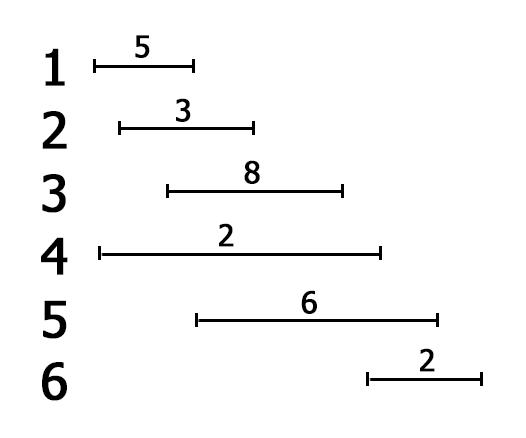
\includegraphics[width=5cm]{09_intervals.png}\\

На выходе мы хотим получить максимальную сумму весов непересекающихся интервалов:

\[
\max\limits_{T\subseteq \left\{ 1,\ldots, n \right\}} \sum\limits_{i\in T}w_i 
\]
\[
T: \forall i<j \implies f_i \leqslant s_j \lor f_j \leqslant s_i
\]

Перебором задача решается за $O(2^n)$

Давайте в качестве первого шага отсортируем по правым концам за $O(n\log n)$.

Введём обозначения:

O --- оптимальное решение

$OPT(i)$ — максимальаня стоимость оптимального решения для первых $i$ интервалов

$OPT(n)$ — Максимальная стоимость оптимального решения длв всех интервалов\\

Пример:

\[
    \mathrm{OPT}(6) = \max\begin{cases}
        \mathrm{OPT}(5), 6\not\in O;\\
        2+ \mathrm{OPT}(3), 6\not\in O; \text{(так как все до третьего не пересекаются с шестым)}
    \end{cases}
\]

Пусть $p(j) = \max\left\{ i<j \mid f_{i}\leqslant s_j\right\}$ --- первый интервал до $j$-го, совместимый с ним (то есть не пересекающийся).

Эффективное вычисление $p$ остается в качестве упражнения.

Тогда общая формула для $OPT$ такова:
\[
    \mathrm{OPT}(i) = \max\begin{cases}
        \mathrm{OPT}(i-1);\\
        w_i+ \mathrm{OPT}(p(i));
    \end{cases}
\]


\begin{algorithm}
	\caption{Подсчёт $OPT(i)$}
	\begin{algorithmic}[1]
		\Function{ComputeOpt}{i}
			\If{\(i = 0\)}
				\State return 0
			\EndIf
			\State return \(\max \{\textsc{ComputeOpt}(i - 1), w_i + \textsc{ComputeOpt}(p(i))\}\)
		\EndFunction
	\end{algorithmic}
\end{algorithm}

Считая, что данные уже отсортированы, получим что сложность равна $O(n)$, но только если мы сохраняем результаты вычислений.
Иначе мы делаем много лишних вычислений, и время будет таким: $T(n) = T(n-1)+T(n-2)+c$.
Очень похоже на числа Фибоначчи, а они растут экспоненциально; это выражение --- тоже.


Значит надо сохранять вычисления в некоторый массив OPT.
Инициализируем его так: 
\[
\mathrm{OPT} = [0, -1, \ldots, -1]
\]

\begin{algorithm}
	\caption{Модифицированный подсчёт $OPT(i)$}
	\begin{algorithmic}[1]
		\Function{ComputeOpt}{i}
			\If{\(OPT(I) < 0\)}
				\State \(OPT[i] = \max \{\textsc{ComputeOpt}(i - 1), w_i + \textsc{ComputeOpt}(p(i))\}\)
			\EndIf
			\State return \(OPT[i]\)
		\EndFunction
	\end{algorithmic}
\end{algorithm}

Вот теперь сложность алгоритма --- $O(n)$

Так как мы вычисляем 1 раз каждый элемент $OPT$, мы можем избавиться от рекурсии:\\

\begin{algorithm}
	\caption{Модифицированный подсчёт $OPT(i)$ без рекурсии}
	\begin{algorithmic}[1]
		\Function{ComputeOpt}{i}
			\State $OPT = [0, -1, \ldots, -1]$
			\For{\(OPT(I) < 0\) \textbf{to} \(n\)}
				\State \(OPT[i] = \max \{OPT[i - 1], w_i + OPT[p(i)]\}\)
			\EndFor
			\State return \(OPT[n]\)
		\EndFunction
	\end{algorithmic}
\end{algorithm}

Как теперь определить, какие именно участки нужно продать?
Можно хранить в $OPT$ на $i$-ом месте необходимые участки, но это замедлит нашу программу (не асимптотически), так как придётся тратить на запись не константное время, а некоторое $O(n)$.
Однако, можно восстановить номера участков по массиву $OPT$:

\begin{algorithm}
	\caption{Восстановление решения}
	\begin{algorithmic}
		\Function{FindSolution}{OPT}
			\State \(T = \emptyset\)
			\State \(i = n\)
			\While{\(i > 0\)}
				\If{\(OPT[i - 1] > w_i + OPT[p(i)]\)}
					\State \(i = i - 1\)
				\Else
					\State \(T = T \cup {i}\)
					\State \(i = p(i)\)
				\EndIf
			\EndWhile
			\State return \(p(i)\)
		\EndFunction
	\end{algorithmic}
\end{algorithm}

\subsection{В общем о динамическом программировании}
Чем оно отличается от ``Разделяй и властвуй''? А тем, что задачи могут пересекаться. Ведь при использовании классического ``разделяй и властвуй'' мы бы получили экспоненциальное решение. 

Для эффективного использования этого принципа необходимы следующие условия:
\begin{itemize}
    \item Небольшое число задач; например, полиномиальное;
    \item Возможность их упорядочить и выразить решения следующих через предыдущие.
\end{itemize}

\subsection{Задача с прошлой лекции --- выравнивание текста}

Дано:\\
$w_1,\ldots, w_n$ --- длины слов.

$c(i, j)$ --- штраф за размещение $w_i,\ldots, w_j$ на одной строке.\\

Преобразуем наше рекурсивное решение в итеративное.

OPT$(i)$ --- оптимальное размещение $w_i, \ldots, w_n$.

OPT(i) = $\min\limits_{i\leqslant j\leqslant n} \left\{ c(i, j)+ \mathrm{OPT}(j+1) \right)\}$.\\

Запишем итеративный алгоритм для этой формулы.
Так как $i$-ая задача зависит от задач с большим индексом, будем заполнять массив с конца.

\begin{algorithm}
	\caption{Выравнивание текста}
	\begin{algorithmic}
		\Function{ComputeOpt}{$w_1, \ldots, w_n$}
			\State \(best = [0] \times n\)
			\State \(OPT = [+\infty] \times (n + 1)\)
			\State $OPT[n + 1] = 0$
			\For{\(i \mathrel{:=} n\) \textbf{downto} 1}
				\For{\(j \mathrel{:=} i\) \textbf{to} n}
					\If{\(c(i, j) + OPT[j + 1] \leqslant OPT[i]\)}
						\State \(OPT[i] = c(i, j) + OPT[j + 1]\)
						\State \(best[i] = j\)
					\EndIf
				\EndFor
			\EndFor
			\State return $OPT[i]$
		\EndFunction
	\end{algorithmic}
\end{algorithm}

Как видно, в данном алгоритме решение строится по ходу, потому что в данном случае это допустимо.

\end{document}
